\documentclass{article}

\usepackage{tabularx}
\usepackage{booktabs}
\usepackage{graphicx}
\usepackage{paralist}
\usepackage{listings}
\usepackage{booktabs}
\usepackage{hyperref}
\usepackage{amsfonts}
\usepackage{amsmath}
\usepackage{color}
\usepackage{fancyhdr}
\usepackage{geometry}
\usepackage{soul}
\usepackage{multirow}
\usepackage{ulem}
\usepackage{float}
\usepackage{tikz}

\title{SRS\\Digital Twin Forest}
\author{Yichen Jiang, Bowen Zhang, Jiacheng Wu, Junhong Chen, Tingyu Shi\\Team 8}

\begin{document}

\maketitle
%%%%%%%%%%%%%%%%%%%%%%%% Revision History %%%%%%%%%%%%%%%%%%%%%%%%%%%%%%%
\newpage
\begin{table}[htp]
\caption{Revision History} 
\begin{tabularx}{\textwidth}{llX}
\toprule
\textbf{Date} & \textbf{Developer(s)} & \textbf{Change}\\
\midrule
Sept 24, 2022 & All team members & Initial Document\\
Sept 26, 2022 & All team members & Update Requirements\\
Sept 29, 2022 & All team members & Revision 0\\

\bottomrule
\end{tabularx}
\end{table}
%%%%%%%%%%%%%%%%%%%%%%%%%%%%%%%%%%%%%%%%%%%%%%%%%%%%%%%%%

\vspace{5cm}

%%%%%%%%%%%% Template Information %%%%%%%%%%%%%%%%%%%%%%%%%%%%%%%
\noindent This document follows \href{https://www.cs.uic.edu/~i440/VolereMaterials/templateArchive16/c\%20Volere\%20template16.pdf}{\textcolor{red}{Volere Template}}.
The following are some modifications that we made to the 
original template:
\begin{itemize}
    \item Our team skipped "Business Data Model and Data Dictionary" because 
    our team will go to the actual forest to measure the data in mid October.
    Also, our team will discuss with Dr. Gonsamo about what data need to be
    added to the virtual forest representation as the project progresses.
    Currently, our team focuses on modelling. We will add this part in Revision
    1.
    \item We added traceability matrices to show relationships between
    functional requirements and non-functional requirements.
    \item We added Likely changes and Unlikely changes.
    \item We added priorities and 
    completion timeline for each functional requirement.
\end{itemize}

%%%%%%%%%%%%% Template Information End %%%%%%%%%%%%%%%%%%%%%%%%%%%%

\newpage

%%%%%%%%%%%%%%Contents%%%%%%%%%%%%%%%%
\tableofcontents
\listoftables
\listoffigures
\cleardoublepage

%%%%%%%%%%% Project Drivers %%%%%%%%%%%%
\section{Project Drivers}
\subsection{The purpose of the Project}
\subsubsection{The User Business or Background of the Project Effect}
A digital twin is a virtual representation of the real world, including physical objects, 
processes, relationships, and behaviors. Elements of a digital twin include data capture
and integration, visualization, advanced analysis including AI, automation, and information
sharing and collaboration. This project can be beneficial for two groups of users.  The first
group of users is forest owners. This project can help them to manage the forest. The 
second group of users is meteorologists. This project can help them to 
do research. \textcolor{red}{Other Team: Expand about how to help meteorologists to do research.}
\subsubsection{Goals of the Project}
\begin{itemize}
    \item Implement the virtual forest, which corresponds to the target natural forest. The model of a single tree is obtained by LiDAR scanning on the field. The final project combines previous models and lab statistics to give a virtual view of the forest. 
    \item Provide basic representations of data, such as age, height, plant density, 
    etc. 
\end{itemize}

\subsection{Stakeholders}
\subsubsection{The client}
\begin{itemize}
    \item Dr. Alemu Gonsamo from School of Earth, Environment and Society McMaster University. (Dr. Gonsamo is the supervisor of this project.)
    \item Dr. Spencer Smith from Computing and Software Department, McMaster University. (Dr. 
    Smith is the professor of the capstone course, and he will give assessments of this project.)
\end{itemize}
\subsubsection{The Customer}
\begin{itemize}
    \item Forest Owners(The final project can be helpful for forest owners to better manage the 
    forest and make decisions)
    \item Meteorologists(The final product can be helpful for researchers to 
    study climate change)
\end{itemize}
\subsubsection{Other Stakeholders}
\begin{itemize}
    \item Dr. Gonsamo's lab members(Graduate students from the lab will provide suggestions and
    data needed to assist this project)
\end{itemize}
\subsubsection{The Hands-On Users of the Product}
The hands-on users of this product are the same as the customers mentioned in section 1.2.2. Users'
responsibilities are also mentioned in section 1.2.2. For subject matter experience, these 
users are masters. For both forest owners and meteorologists, they are definitely
familiar with the real forest and our product can help them better do
their jobs. From the point of technology, we assume that they 
have little experience with virtual representation
technologies.
\subsubsection{Personas}

\begin{itemize}
    \item Dr. Aly is a 55-year-old assistant professor working in a university, living with his family near his lab. His research mainly focuses on remote sensing of vegetation, global change ecology, and climate change impact. His research is supported by an association of several forest owners, who are willing to let Dr. Aly locate part of the researches and collect needed information in their forest. If he needs to go to the field that day, the typical schedule of him is to get up at 6 am, take 90 minutes to commute to the target forest with some students he supervises, collect and record data there, and come back to his lab with another 90 minutes. 
    
    Dr. Aly's goals are to find a convenient way to free him from frequent commuting and to look for a new method to manage and visualize all the significant data for a purpose of teaching. 
    
    \item Mrs. Miller owns 40-acre land including a 2-acre forest. She is now 36 years old and lives with her husband, who works as a financial analyzer, in Toronto. She runs a coffee house as a full-time job and drives to her forest every two months to check everything's fine. Though she cares about her forest, spending over three days every two months going through every area seems impossible for her, she would love to have a new method to manage her forest and get updated information regularly, in order to make better strategies for the forest. 
\end{itemize}


\subsubsection{Priorities Assigned to Users}
\begin{itemize}
    \item Key Users: Dr. Gonsamo, Forest owners, meteorologist
    \item Secondary Users: Dr. Smith, Lab members
\end{itemize}
\subsubsection{User Participation}
\begin{itemize}
    \item Dr. Smith: Dr. Smith will provide suggestions about project management, project 
    documents and project technologies like git.
    \item Dr. Gonsamo: Dr. Gonsamo will provide business knowledge(forest data), 
    interface prototyping and usability requirements for this project. Since Dr. Gonsamo is 
    a meteorologist, he can also provide suggestions for meteorologists.
    \item Lab members: Lab members will help this project by providing some business knowledge
    about the forest.
    \item Forest Owners: Forest owners can provide commercial data about the forest. Commercial
    data include tree-cutting data, annual profits, etc.
\end{itemize}
\subsubsection{Maintenance Users and Service Technicians}
The project members will be responsible for maintaining and changing the product.
%%%%%%%%%%% Project Drivers End %%%%%%%%%%


%%%%%%%%%% Project Constraints %%%%%%%%%%%%
\section{Project Constraints}
\subsection{Mandated Constraints}
\subsubsection{Solution Constraints}
\begin{itemize}
    \item Scanning Technology: Our team will use Light Detection and Ranging(LiDAR) method
    to scan physical objects in the forest. This is a kind of Laser Scanning technology. 
    We determined to use this technology for three reasons. First, LiDAR sensors
    are accessible because they are common among Apple devices like iPhone or iPad. The 
    second reason is that LiDAR sensors can provide accurate scanning. The third reason
    is that LiDAR allows to scan large areas within a short period of time.
    \item Modeling Technology: Our team will use Unity for the modeling task. The Unity version will be 2021.3. Our team members use different platforms(Windows or MacOS). Unity is 
    suitable for our team because it is a cross-platform software. Also, Unity has existing packages which can speed up our modeling process.
    \item Project Documents Technology: Our team will use \LaTeX for our documents.
    \item Project Cooperation Technology: Our team will use GitHub to cooperate.
    \item Code Testing Technology: VS2019 will be used for the unit test. The team will create a unit test project (.NET Framework) that contains MSTest unit tests.
    \item Code Coverage Testing Technology: The JetBrains dotCover is a code coverage tool that integrates with VS2019. It can execute and run coverage analysis for unit tests in Visual Studio.
\end{itemize}
\subsubsection{Implementation Environment of the Current System}
The product will be installed in different operating systems such
as Windows, MacOS, iPadOS, iOS, and Android. The rationale for this is that users may use our product on different platforms.
\subsubsection{Partner or Collaborative Applications}
N/A(Our product is an independent product)
\subsubsection{Off-the-Shelf Software}
\begin{itemize}
    \item LiDAR: iPad Pro LiDAR should be used to scan the forest and collect data
    for modelling.
    \item Unity: Unity should be used for modelling and post-processing.
    \item Agisoft metashape: It should be used for modelling.
\end{itemize}
\subsubsection{Anticipated Workplace Environment}
Both indoor and outdoor are possible workplace environments. In order to 
improve the convenience for outdoor workplace environments, 
the product should be compatible with mobile devices such
as cell phones or tablets.
\subsubsection{Schedule Constraints}
Please check our project schedule \href{https://github.com/wuj187/DigitalTwinCAS/tree/main/docs/DevelopmentPlan/Project_Schedule}{\textcolor{red}{here}}. The following are deadlines for demonstrations:
\begin{itemize}
    \item Proof of Concept Demonstration: 2022, Nov, 14
    \item Final Demonstration: 2023, Mar, 20
\end{itemize}
\subsubsection{Budget Constraints}
Total expenses should not exceed \$750.
\subsubsection{Enterprise Constraints}
N/A This project is not invested by any enterprise.
\subsection{Naming Conventions and Definitions}
\begin{itemize}
    \item LiDAR: Light Detection and Ranging(Scanning Technology)
    \item Plot: A square shaped area in the forest. There are 13 plots in total. 
    \item Target Forest: The natural forest modelled in this product.
    \item Digital Twin Forest: The virtual representation of the target forest.
    \item Update local data: The users are allowed to update any data on their own device. The update made by a user will not be updated to the other users.
    \item Update official data: The developing team would release updates regularly. The update made by the developing team can be updated to all users if they accept the latest version.
    \item Overall forest data: These are data for the whole forest. For example,
    these data may include overall $CO_2$ concentration or plant density of the whole
    forest.
    \item Forest plot data: The target forest is separated into 13 plots. Plot forest
    data
    has the same data types as the overall forest data, however, all the data are for
    a specific forest plot.
    \item Tree parameters: Tree parameters include data such as tree ages,
    perimeters,
    heights, species, etc.
\end{itemize}

\subsection{Relevant Facts and Assumptions}
\subsubsection{Relevant Facts}
\begin{itemize}
    \item Forest data keep changing all the time, but our 
    system will only update weekly. Therefore, the 
    system may not be able to reflect the most accurate data. 
    However, since the forest data will not change dramatically
    within a short period of time, the system should be 
    close to the real forest.
    \item The product can be beneficial for meteorologists to do research.
    \item The product can be beneficial for forest owners 
    to better manage the forest.
\end{itemize}
\subsubsection{Business Rules}
N/A
\subsubsection{Assumptions}
\begin{itemize}
    \item The scanning devices are available.
    \item Drones can be used for large area scanning.
    \item Unity and required toolboxes 
    should be accessible to all developers'
    devices.
    \item Users will use our product on Windows, MacOS, iOS, iPadOS,
    or Android.
    \item Forest data will not change dramatically within a 
    short period of time. 
    \item Virtual forest should be updated weekly for the 
    first year.
\end{itemize}
%%%%%%%%%%%% Project Constraints End %%%%%%%%%


%%%%%%%%%%% Functional Requirements %%%%%%%%%%%%
\section{Functional Requirements}
\subsection{The Scope of the Work}
\subsubsection{The Current Situation}
Currently, digital twin technologies are being utilized in many
areas, such as Aerospace and Aeronautics, manufacturing, automotive, etc. For more detailed information, please check paper \href{https://github.com/wuj187/DigitalTwinCAS/blob/main/refs/DT_Applications.pdf}{\textcolor{red}{\textit{Applications of Digital Twin across 
Industries: A Review}}} in our reference folder. This paper talks about 
many applications of digital twin technologies in different areas.\\
After searching online, we found a similar product from Tietoery
Company called \href{https://www.tietoevry.com/en/industries/forest-pulp-paper-and-fibre/forest-solutions/wood-and-fibre-ecosystem-and-integration/digital-forest-twin/}{\textcolor{red}{Digital Forest Twin}}.
According to its introduction, this product can 
be accessed using head-mounted devices or
web browsers, which is different from our product. Also, 
from the company's website, we can know little details about how
 this product works. Therefore, our team does not know too much
 about existing business processes.
 \newpage
\subsubsection{The Context of the Work}
The following is the context of use diagram:
\begin{figure}[H]
\begin{center}
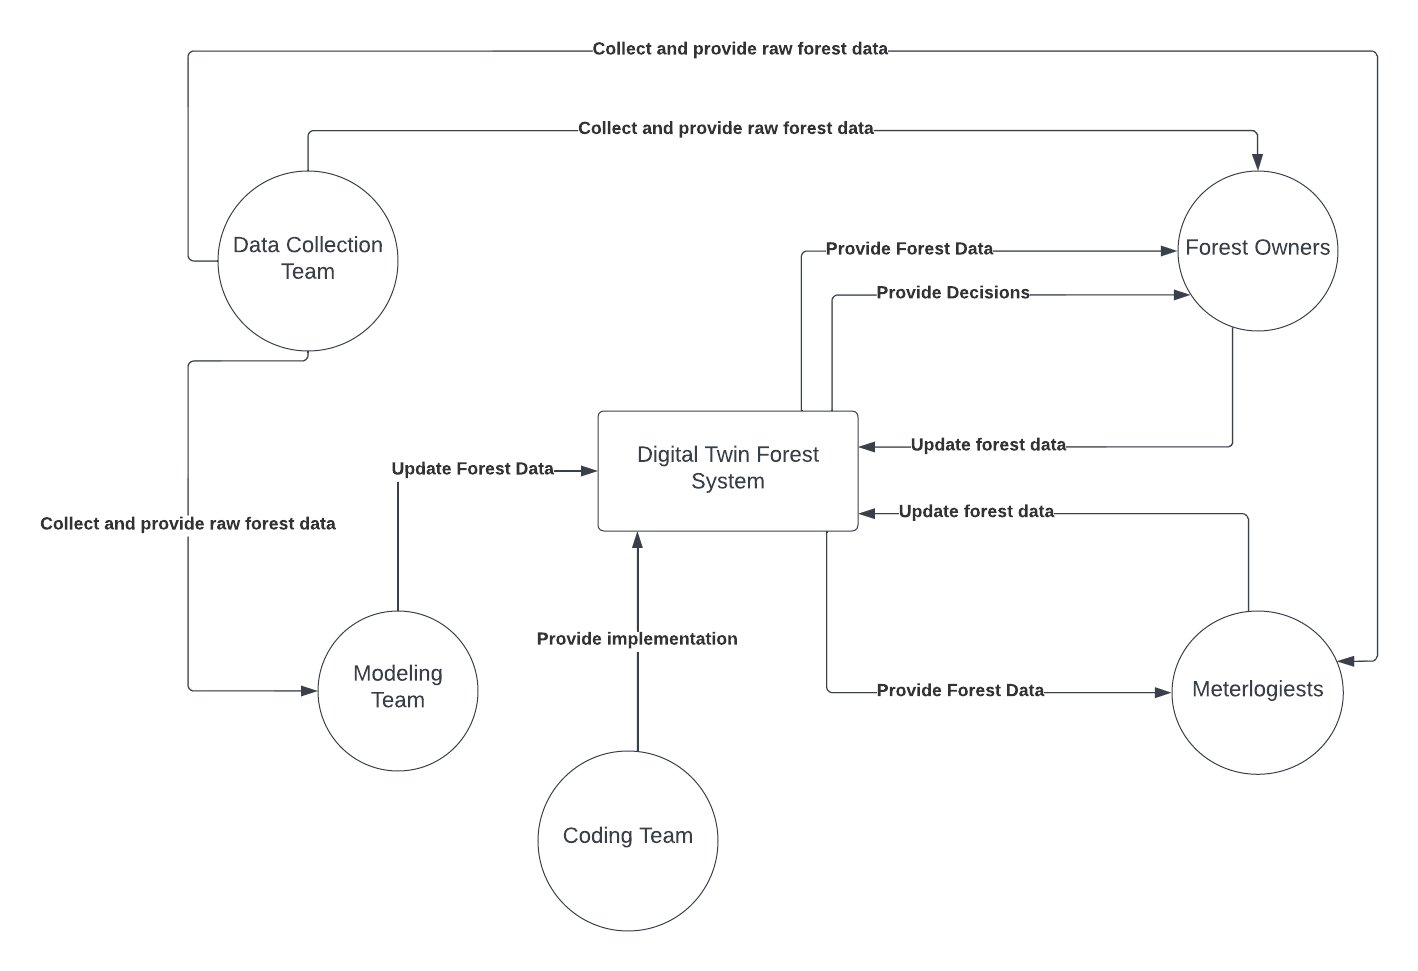
\includegraphics[scale=0.7]{SRS_Pictures/Context_Use.png}
\end{center}
\caption{Context Diagram}
\end{figure}
\noindent \textcolor{red}{Other Team: Differentiate the responsibilities/roles between coding teaming
and modelling team}\\
\noindent If the above picture is not clear, please download the picture \href{https://github.com/wuj187/DigitalTwinCAS/blob/main/docs/SRS/SRS_Pictures/Context_Use.png}{\textcolor{red}{here}}. \\

\noindent Forest data includes the following:
\begin{itemize}
    \item Forest atmosphere data (eg. $CO_2$ concentration)
    \item Forest measurements (eg. distance between different trees)
    \item Tree parameters(eg. height, trunk perimeter, age, speices)
    \item Forest soil data
    \item Plant density
\end{itemize}
As the project progresses, we may add more data to our virtual forest representation.

\subsubsection{Work Partitioning}
\begin{table}[H]
\caption{Business Event List} 
\begin{tabularx}{\textwidth}{XXX}
\toprule
\textbf{Event Name} & \textbf{Input and Output} & \textbf{Summary of BUC}\\
\midrule
Forest scanning & Forest data(in) & Scan the forest and generate data for modelling.\\
Import models & Forest models(in) & Edit and upload new models to the system.\\
Code implementation & System modules(in) & Add new modules to the system.\\
Update data & Forest Data(in) & Replace the old data in the system with new data.\\
Data visualization & Forest Data(output) & The system demonstrates the organized data to the users.\\
Decision Making & Forecast and suggestions (output) & The system generates reports based on the given data.\\
\bottomrule
\end{tabularx}
\end{table}

\newpage
\subsubsection{Specifying a Business Use Case (BUC)}
The following is an activity diagram to indicate how users can check various data
from the system\\
\begin{figure}[H]
    \centering
    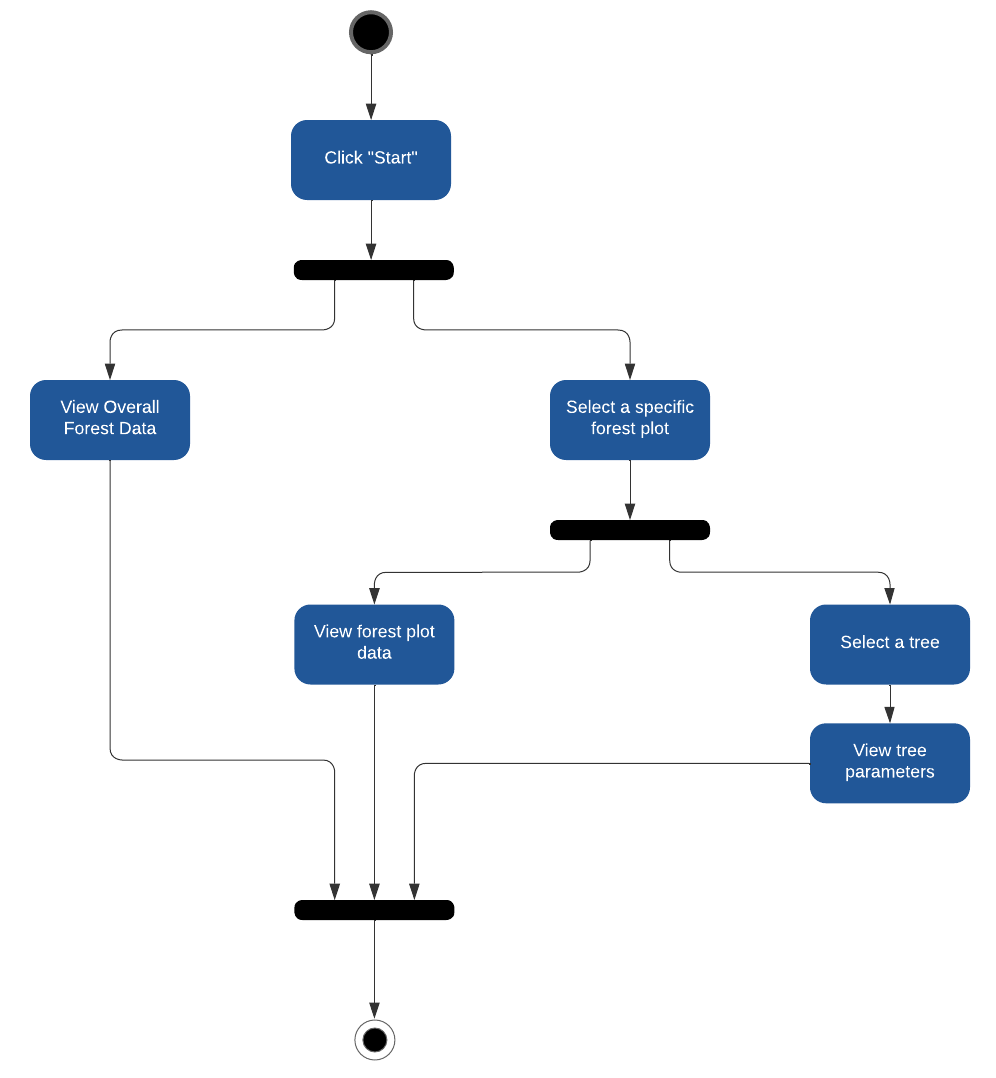
\includegraphics[scale=0.8]{SRS_Pictures/Activity_Diagram.png}
    \caption{An activity diagram to show how users can check data}
\end{figure}
\noindent If the above picture is not clear, please download the picture \href{https://github.com/wuj187/DigitalTwinCAS/blob/main/docs/SRS/SRS_Pictures/Activity_Diagram.png}{\textcolor{red}{here}}.

\subsection{The Scope of the Product}
\subsubsection{Product Boundary}
\begin{figure}[H]
    \centering
    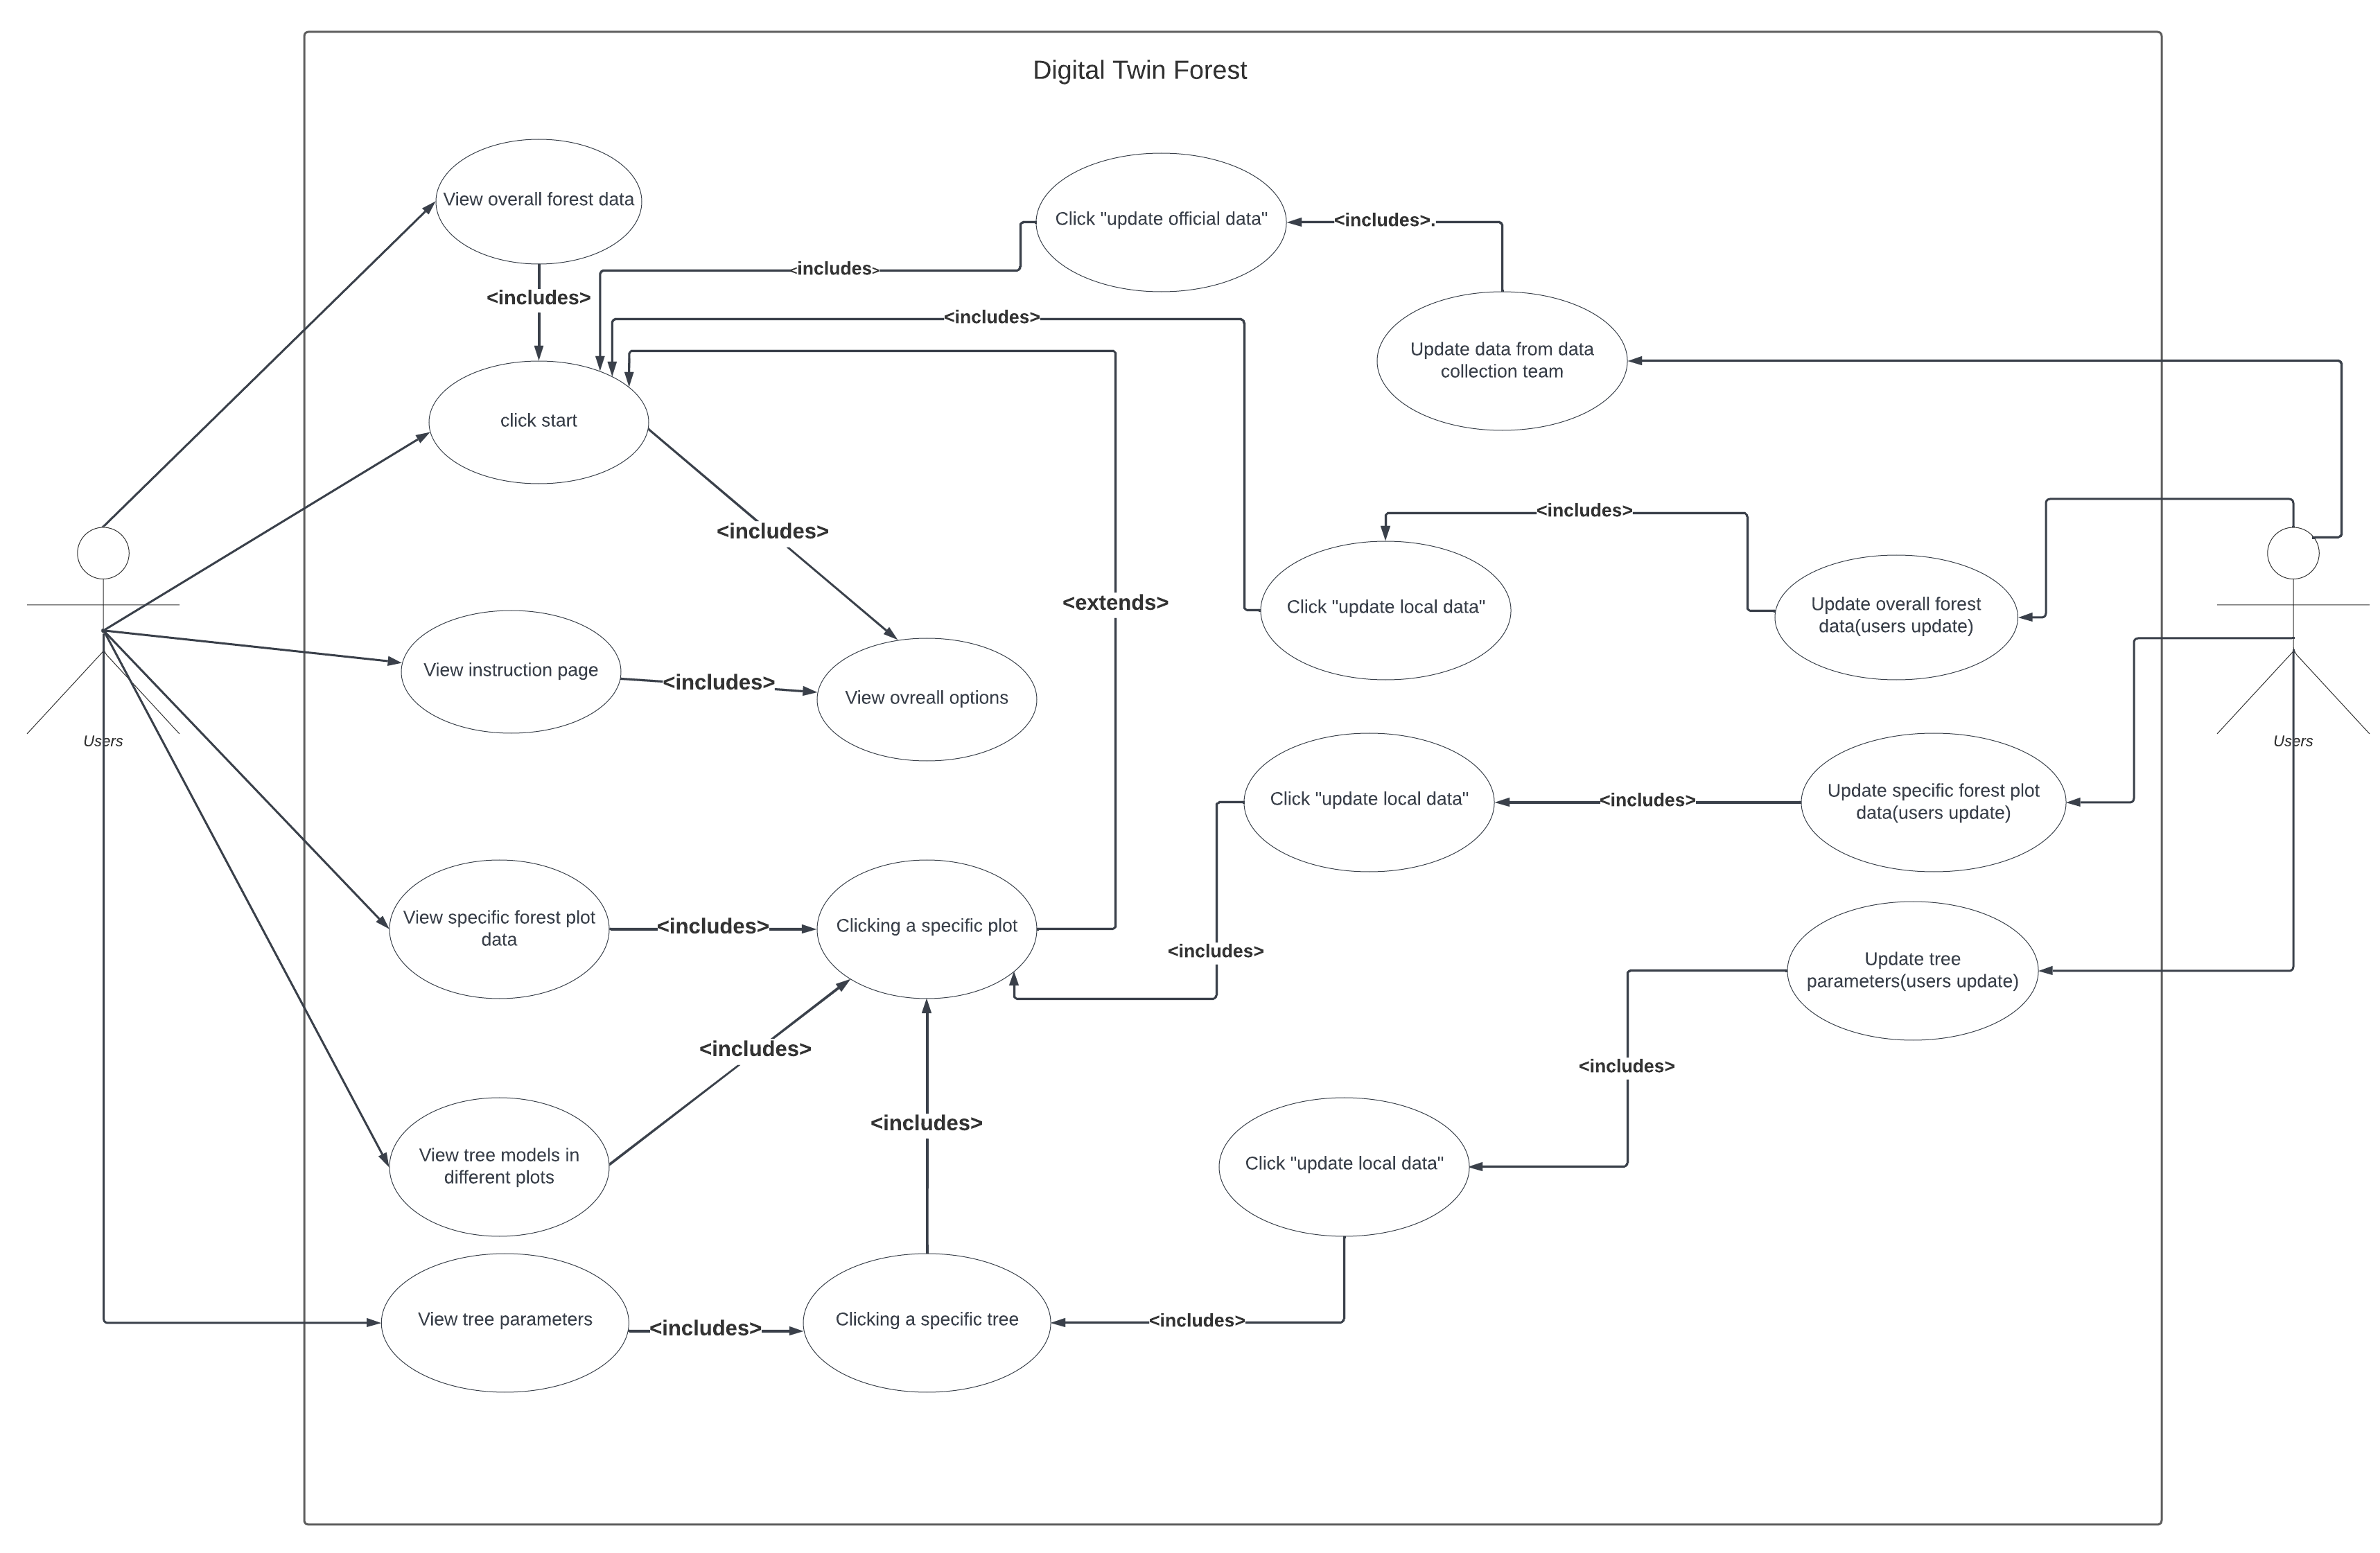
\includegraphics[scale=0.3]{SRS_Pictures/Use_Case.png}
    \caption{Use Case Diagram}
\end{figure}
\noindent If the above picture is not clear, please download the picture \href{https://github.com/wuj187/DigitalTwinCAS/blob/main/docs/SRS/SRS_Pictures/Use_Case.png}{\textcolor{red}{here}}.

\subsubsection{Product Use Case Table}
\begin{enumerate}
    \item PUC Name: View overall forest data\\
    Actor: Users\\
    Input: Users click "start" at the beginning of the application.\\
    Output: Overall forest data appear in the windows on two sides of the screen. 
    \item PUC Name: Click start\\
    Actor: Users\\
    Input: Users click "start" at the beginning of the application.\\
    Output: 13 plots and overall forest data appear on the screen.
    \item PUC Name: View instruction page\\
    Actor: Users.\\
    Input: Users click "Instruction" at the beginning of the application.\\
    Output: The instruction page appears on the screen. 
    \item PUC Name: View specific forest plot data\\
    Actor: Users.\\
    Input: Users click a specific forest plot.\\
    Output: Forest data of a specific plot appear in the windows on two sides of
    the screen. 
    \item PUC Name: View tree models in different plots\\
    Actor: Users.\\
    Input: Users click a specific forest plot.\\
    Output: Tree models of a specific plot appear on the screen.
    \item PUC Name: View tree parameters\\
    Actor: Users.\\
    Input: Users click a specific tree.\\
    Output: Tree parameters appear in a window beside the tree.
    \item PUC Name: Update data from data collection team\\
    Actor: Users.\\
    Input: Users click "update official data".\\
    Output: All the data(including overall forest data, forest plot data and tree 
    parameters) will be synchronized with the official data collected from the 
    data collection team.
    \item PUC Name: Update overall forest data(Users update)\\
    Actor: Users.\\
    Input: Users click "update local data" after clicking "start".\\
    Output: A window appears on the screen to let users update overall
    forest data.
    \item PUC Name: Update forest plot data\\
    Actor: Users.\\
    Input: Click "update local data" in a specific forest plot.\\
    Output:  A window appears on the screen to let users update
    forest plot data.
    \item PUC Name: tree parameters\\
    Actor: Users.\\
    Input: Click "update local data" in tree information windows.\\
    Output:  A window appears on the screen to let users update tree 
    parameters.
\end{enumerate}



\subsection{Functional Requirements}
\textcolor{red}{All the rationale and fit criteria are not revised for FR.}
\begin{enumerate}[FR1]
	\item The product shall \textcolor{red}{\st{display} provide an option to display} basic
	 instructions. \textcolor{red}{\st{when users access to the product for the first time}}\\
	\textbf{Rationale}: Users might not be familiar with our product especially when they use 
	it for the first time.\\
	\textbf{Fit Criterion}: A basic instruction 
	option shows up on the user interface after the software is launched. 
	
	\item The product shall \textcolor{red}{provide a way to} allow users \textcolor{red}{\st{to click
	 a start button}} to start the virtual tour.\\
	\textbf{Rationale}: The user would need a clear signal to get started.\\
	\textbf{Fit Criterion}: A 'start' button is displayed on the home page of the application.
	
	\item The product shall load the forest model when users \textcolor{red}{\st{clicks start} give
	the system inputs to start.}\\
	\textbf{Rationale}: The clicking of 'start' indicates the user has been through the instruction and is ready to use our product. The product can now initialize the functions by loading the model.\\
	\textbf{Fit Criterion}: Once the user select 'start', the data of the forest is loaded.
	
	\item The product shall display the \textcolor{red}{percentage of }progress \textcolor{red}{\st{bar}} while \textcolor{red}
	 {the forest models are being loaded.} \\
	\textbf{Rationale}: The product should give feedback on the action of clicking 'start'. The loading might take seconds and a progress bar helps when the user's waiting. \\
	\textbf{Fit Criterion}: A dynamic progress bar will be displayed when the forest is loading.
	
	\item The product shall display a full view of the \textcolor{red}{overall} digital twin
	forest.\\
	\textbf{Rationale}: Users might not be aware of the overall information and the overview of the forest that the product simulates.\\
	\textbf{Fit Criterion}: 13 complete plots of the forest with highlighted borders will show up together when the user zooms out the interface.
    
    \item The product shall allow users to minimize the user interface\textcolor{red}{ (User 
    interface includes windows that present forest data)}. \\
    \textbf{Rationale}: The user might want to pay more attention to the model instead of information related to it. Minimizing the user interface allows the user to do so. \\
	\textbf{Fit Criterion}: The windows of the user interface will be minimized to the side of the screen once the user clicks the \textit{minimized} button on the user interface.
	
	\item The product shall \textcolor{red}{be able to} display \textcolor{red}{\st{a menu to show
	 specific data} forest plot data} when users \textcolor{red}{\st{clicks on each} select
	 a specific forest} plot.\\
	\textbf{Rationale}: After the user has located a specific plot, he or she should be able to access to related information. And the most intuitive and convenient method to do so would be clicking. \\
	\textbf{Fit Criterion}: After the user clicks on a specific plot, windows containing information about that plot shall be displayed on both sides of the screen.
	
	\item The product shall allow users to \textcolor{red}{\st{click} select} a specific tree in order
	 to view related information\textcolor{red}{(Tree Parameters)}.\\
	\textbf{Rationale}: It allows users to see the related information of a specific tree in detail.\\
	\textbf{Fit Criterion}: After the user enters a specific plot and clicks on a specific tree. windows containing information about that kind of tree shall be displayed on both sides of the screen. 
	
	\item The product shall display the \textcolor{red}{\st{overall} forest} data\textcolor{red}{(both 
	overall forest data and forest plot data)} \textcolor{red}{\st{of the forest on both sides of the
	 screen} without interrupting users viewing forest models}.\\
	\textbf{Rationale}: The product should display the important data that our users might care about on the user interface while not letting the information interrupt the display of the model. Therefore, it should distribute the information on both sides.\\
	\textbf{Fit Criterion}: When the full view of the forest is displayed, windows containing the overall information about the forest shall be shown on both sides of the screen. 
	
	\item The product shall allow users to zoom in and out of the \textcolor{red}{\st{model} the 
	digital twin forest}.\\
	\textbf{Rationale}: The user might need to zoom in to locate a specific plot or zoom out for a fuller view of the forest. \\
	\textbf{Fit Criterion}: When the user scrolls forward the scroll wheel of the mouse, the map shall be zoomed in. When the user scrolls backward, the map shall be zoomed out. 
	
	\item The product shall allow users to change the point of view. \\
	\textbf{Rationale}: The users might need to observe the forest from different perspectives.\\
	\textbf{Fit Criterion}: The user's point of view shall change when the user moves the mouse and scrolls the scroll wheel.
	
	\item \textcolor{red}{\st{The product shall display the information on separate pages when the
	 content does not fit on one page.} The product shall provide a way to present all the data when
	  the amount of data is huge.}\\
	\textbf{Rationale}: The amount of information might not fit on a single page. Instead of
	 compromising the user interface and minimizing the font size, displaying the information on
	  several pages would be a better choice.\\
	\textbf{Fit Criterion}: Several pages will show up when showing information with very long content.
	
	\item The product shall allow users to turn pages if the interface has multiple pages. \\
	\textbf{Rationale}: The user should be able to turn pages to switch among different sections of information.\\
	\textbf{Fit Criterion}: When showing multiple pages, page turn buttons shall be on each page. When the user clicks on the forward page turn button, the page shall display the previous information. When the user clicks on the backward page turn button, the page shall display the subsequent information.
	
	\item The product shall allow users to go back to the overall view \textcolor{red}{of the digital
	twin forest} when \textcolor{red}{\st{focusing on} they are viewing} a certain forest plot.\\
	\textbf{Rationale}: Users might need to go back to see the overview of the forest and see some
	 overall information about the forest.  \\
	\textbf{Fit Criterion} The full view of the forest shall show up when the user scrolls backward the
	 scroll wheel of the mouse.
	
	\item The product shall \textcolor{red}{provide ways to }allow users to \textcolor{red}{\st{click
	 an exit button and}} quit the product.\\
	\textbf{Rationale}: The user would need a clear signal to exit.\\
	\textbf{Fit Criterion}: Once the user clicks on the 'exit' button, the application shall quit and the process of the software shall be terminated.
    
    \item The product shall allow users to update \textcolor{red}{\st{the information about the forest
     and trees} forest data(both overall forest data and forest plot data) and tree parameters}.\\
	\textbf{Rationale}: In order to let the application show the latest information, it's necessary for
	 users to upload the renew the information and statistics about the forest by themselves.\\
	\textbf{Fit Criterion}: After the user uploads the latest information, the virtual forest shall
	 display this latest information. 
	
	\item The product shall allow users to choose to update the product or not when a new
	 version is released. \textcolor{red}{Update may include the latest forest data and
	 some new functions and features of the product.}\\
	\textbf{Rationale}: Our product relies deeply on the latest information to give reasonable
	 references. The user can choose to update to the latest version when any version is released.\\
	\textbf{Fit Criterion}: The product should overwrite any modification made by users and update all
	 the information corresponding to the latest released version of our product.
\end{enumerate}

\subsection{Priority and Timeline}
\begin{table}[H]
\centering
\begin{tabular}{|lll|}
\hline
\multicolumn{3}{|l|}{Priority and Timeline}                                                                                                                                 \\ \hline
\multicolumn{1}{|l|}{\begin{tabular}[c]{@{}l@{}}Functional\\ Requirements\end{tabular}} & \multicolumn{1}{l|}{Priority}        & Timeline                                   \\ \hline
\multicolumn{1}{|l|}{FR1}                                                               & \multicolumn{1}{l|}{low priority}    & October 20th, 2022 to October 27th, 2022   \\ \hline
\multicolumn{1}{|l|}{FR2}                                                               & \multicolumn{1}{l|}{meduim priority} & October 27th, 2022 to November 3rd, 2022   \\ \hline
\multicolumn{1}{|l|}{FR3}                                                               & \multicolumn{1}{l|}{high priority}   & January 26th, 2022 to February 9th, 2023   \\ \hline
\multicolumn{1}{|l|}{FR4}                                                               & \multicolumn{1}{l|}{low priority}    & November 10th, 2022 to November 17th, 2022 \\ \hline
\multicolumn{1}{|l|}{FR5}                                                               & \multicolumn{1}{l|}{meduim priority} & December 15th, 2022 to January 12th, 2023  \\ \hline
\multicolumn{1}{|l|}{FR6}                                                               & \multicolumn{1}{l|}{low priority}    & November 24th, 2022 to December 1st, 2022  \\ \hline
\multicolumn{1}{|l|}{FR7}                                                               & \multicolumn{1}{l|}{high priority}   & February 9th 2023 to February 16th, 2023   \\ \hline
\multicolumn{1}{|l|}{FR8}                                                               & \multicolumn{1}{l|}{high priority}   & February 16th, 2023 to February 23rd, 2023 \\ \hline
\multicolumn{1}{|l|}{FR9}                                                               & \multicolumn{1}{l|}{high priority}   & November 17th, 2022 November 24th, 2022    \\ \hline
\multicolumn{1}{|l|}{FR10}                                                              & \multicolumn{1}{l|}{high priority}   & January 12th, 2023 to January 15th, 2023   \\ \hline
\multicolumn{1}{|l|}{FR11}                                                              & \multicolumn{1}{l|}{high priority}   & January 15th, 2023 to January 19th, 2023   \\ \hline
\multicolumn{1}{|l|}{FR12}                                                              & \multicolumn{1}{l|}{low priority}    & December 1st, 2022 to December 8th, 2022   \\ \hline
\multicolumn{1}{|l|}{FR13}                                                              & \multicolumn{1}{l|}{low prirority}   & December 8th, 2022 to December 15th, 2022  \\ \hline
\multicolumn{1}{|l|}{FR14}                                                              & \multicolumn{1}{l|}{high priority}   & January 19th, 2023 to January 26th, 2022   \\ \hline
\multicolumn{1}{|l|}{FR15}                                                              & \multicolumn{1}{l|}{meduim priotity} & November 3rd, 2022 to November 10, 2022    \\ \hline
\multicolumn{1}{|l|}{FR16}                                                              & \multicolumn{1}{l|}{high priority}   & February 23rd, 2023 to March 9th, 2023     \\ \hline
\multicolumn{1}{|l|}{FR17}                                                              & \multicolumn{1}{l|}{high priority}   & March 9th, 2023 to March 23rd, 2023        \\ \hline
\end{tabular}
\caption{Functional Requirements Priority Table}
\end{table}

\textcolor{red}{
The following are FR related comments from other team
\begin{itemize}
\item mention more about how the data the forest/data will be constructed, consumed or inputted
into the system.
\item FR2 and FR3 are ambitious. In FR2, your 'start' button on the main page will redirect your users to the virtual tour page. In FR3, your 'start' button will start the data loading process. Is the 'start' button in FR3 different from your FR2 'start' button? I will suggest you use two different names for the buttons to distinguish the two functions.
\item FR16:
What does it mean for the latest information? Is it data, user interface, new functions, or something else? You should classify it so that the developer can know the latest information they need to provide to the users.
\end{itemize} 
}

%%%%%%%%%%%%% Functional Requirements End %%%%%%%%%%%



%%%%%%%%%%%%% Non-functional Requirements %%%%%%%%%%%%%
\section{Nonfunctional Requirements}
\subsection{Look and Feel Requirements}
\subsubsection{Appearance Requirements}
\begin{enumerate}
    \item[LF1.1] The product shall have a goal that all modules adhere to. \\
    \textbf{Rationale}: The system can be consistent and coherent if all modules focus on one goal, and
     it's easy for users to understand the function of the system.\\
    \textbf{Fit criterion}:  There are at least 8 modules that serve one function in every 10 modules.
   
    \item[LF1.2] \textcolor{red}{\st{The goal of the product shall be to display a lifelike forest to
     the users.} The digital twin forest should be lifelike compared with the target
     forest.}\\
    \textbf{Rationale}: The graphic quality can optimize users' experiences.\\
    \textbf{Fit criterion}: Among \textcolor{red}{\st{10 samples of users who use it for the first
     time} all the sample users during the testing phase}, \textcolor{red}{\st{8} 80\%} of them agree
      \textcolor{red}{\st{trees} the digital twin forest} is lifelike.
\end{enumerate}
\subsubsection{Style Requirements}
\begin{enumerate}[LF2.1]
    \item The product shall appear authoritative based on the real forest.\\
    \textbf{Rationale}: The product is reliable only if it's based on real data.\\
    \textbf{Fit criterion}: The data in our project will not exceed a relative error of 
    5\%.
    
    \item The product shall appear professional.\\
    \textbf{Rationale}: A project is more convincing if it looks professional.\\
    \textbf{Fit criterion}: Among \textcolor{red}{\st{10 samples of users} all sample users during the 
    testing phase}, at least \textcolor{red}{\st{8} 80\% of them} think the system is professional.
\end{enumerate}
\subsection{Usability and Humanity Requirements}
\subsubsection{Easy of Use Requirements}
\begin{enumerate}[UH1.1]
    \item The product instructions shall be easy to understand.\\
    \textbf{Rationale}: Clear instructions can take users less time to learn to use this product.\\
    \textbf{Fit criterion}: Among \textcolor{red}{\st{10 users} all the sample users during the 
    testing phase}, at least 80\% of them can learn how to use the system within half an hour.
\end{enumerate}
\subsubsection{Personalization and Internationalization Requirements}
\begin{enumerate}[UH2.1]
    \item The product shall use English only.\\
    \textbf{Rationale}: English is a general language that most users know.\\
    \textbf{Fit criterion}: 100\% of the text is in English.
\end{enumerate}
\subsubsection{Learning Requirements}
\begin{enumerate}[UH3.1]
    \item The instructions of the product shall be displayed on the instruction page.\\
    \textbf{Rationale}: Users can easily access the instructions on the instruction page.\\
    \textbf{Fit criterion}: Instructions option is displayed on the main page, after clicking it users can see the instructions shown on the instruction page.
\end{enumerate}
\subsubsection{Understandability and Politeness Requirements}
\begin{enumerate}[UH4.1]
    \item The product shall use \textcolor{red}{\st{symbols} icons} to highlight core functions.\\
    \textbf{Rationale}: Highlight can make users notice the core function of the system.\\
    \textbf{Fit criterion}: Among \textcolor{red}{\st{10} all the sample users during the 
    testing phase}, over 80\% of them can notice and 
    \textcolor{red}{understand} the \textcolor{red}{\st{highlight} icons}.
    
    \item The product shall use icons that are appealing to all ages.\\
    \textbf{Rationale}: Icons can improve users' experience.\\
    \textbf{Fit criterion}: Among \textcolor{red}{\st{10} all the sample users during the 
    testing phase}, over 80\% of them think the icons are appealing.
\end{enumerate}
\subsubsection{Accessibility Requirements}
\begin{enumerate}[UH5.1]
    \item The product shall be usable by people who are able to use a \textcolor{red}{\st{computer}
     keyboard} and a mouse.\\
    \textbf{Rationale}: The interface of the system shall be consistent with other software (e.g use a
     mouse and keyboard).\\
    \textbf{Fit criterion}: 100\% of the actions can be done with a mouse and a keyboard.
    
    \item The product's user interface should be easy to learn.\\
    \textbf{Rationale}: A neat and clean user interface can take users less time to learn to use.\\
    \textbf{Fit criterion}: Among all the sample users during the testing phase, over 80\% of them
     can learn how to use the system within half an hour.
\end{enumerate}
\subsection{Performance Requirements}
\subsubsection{Speed and Latency Requirements}
\begin{enumerate}
    \item[PR1.1] The product shall respond to user \textcolor{red}{\st{actions} requests} quickly.\\
    \textbf{Rationale}: Quick response can improve users' experience.\\
    \textbf{Fit Criterion}: The system can respond within 2 seconds \textcolor{red}{\st{for 23 hours
     out of 24 hours} for all the user requests}.
    
    \item[PR1.2] The product shall run at high FPS.\\
    \textbf{Rationale}: Smooth display can improve users' experience.\\
    \textbf{Fit Criterion}: The system should run at least 30 frames per second over 80\% of the time.
    
    \item[PR1.3] The product shall be able to load the models fast.\\
    \textbf{Rationale}: Less wait time for users can improve users' experience.\\
    \textbf{Fit Criterion}: The waiting time will not exceed 10 seconds 100\% of the time.
\end{enumerate}
\subsubsection{Safety-Critical Requirements}
N/A
\subsubsection{Precision or Accuracy Requirements}
\begin{enumerate}[PR3.1]
    \item Data displayed on the screen shall be accurate.\\
    \textbf{Rationale}: The data is supposed to be reliable.\\
    \textbf{Fit Criterion}: \textcolor{red}{\st{100\% of the data in this system are in two decimals}
    All the data in the system should have at most 5\% relative errors compared with the target
    forest data}.\\
 
   
    \item \textcolor{red}{\st{The relative error of each model shall be small. \\
    \textbf{Rationale}: The data is supposed to be reliable.\\
    \textbf{Fit Criterion}: The relative error will not exceed 30\% for each data.}}\\
    
\end{enumerate}
\subsubsection{Reliability and Availability Requirements}
\begin{enumerate}[PR4.1]
    \item The product shall be available whenever users access to it.\\
    \textbf{Rationale}: The product is reliable if it's available most of the time.\\
    \textbf{Fit criterion}: The system is required to work \textcolor{red}{\st{over 23 hours in a
     day} all the time}.
    
    \item The product shall \textcolor{red}{\st{not} avoid} crashing while running.\\
    \textbf{Rationale}: Stable running environment can make the product more reliable.\\
    \textbf{Fit Criterion}: The system shall not crash over once out of 100 hours of running.\\
\end{enumerate}
\subsubsection{Robustness or Fault-Tolerance Requirements}
\begin{enumerate}[PR5.1]
    \item The product shall be able to run locally.\\
    \textbf{Rationale}: The product can be more reliable if it runs locally.\\
    \textbf{Fit Criterion}: The product can \textcolor{red}{\st{run normally for 23 hours for every 24
     hours} perform all the functions without internet connection}.
\end{enumerate}
\subsubsection{Capacity Requirements}
\begin{enumerate}[PR6.1]
    \item The software size shall not be too large.\\
    \textbf{Rationale}: Less size can make the software more portable.\\
    \textbf{Fit Criterion}: The size of the software shall not exceed 10 GB.
\end{enumerate}
\subsubsection{Scalability or Extensibility Requirements}
\begin{enumerate}[PR7.1]
    \item New components shall be easily added to the product in the future version.\\
    \textbf{Rationale}: If the components can be added easily, we can update the content and modify the system more easily.\\
    \textbf{Fit Criterion}: \textcolor{red}{\st{A programmer will not spend over one day adding a
     feature to the system} Adding new features or functions shall not need to modify over 
     two existing modules}.\\
\end{enumerate}
\subsubsection{Longevity Requirements}
\begin{enumerate}[PR8.1]
    \item \textcolor{red}{\st{The product shall be expected to operate within the maximum maintenance
     budget for a minimum of one year} The developers should ensure the product having 
     satisfying qualities for at least a year after releasing}.\\
    \textbf{Rationale}: The developer team is mandatory to run the project for at least one year, and
     later plan is to be determined.\\
    \textbf{Fit Criterion}: \textcolor{red}{\st{The developer team must pay enough effort and spend the
     necessary budget on
     this product for at least one year, to ensure the product reaches a satisfying quality. This is to
      say, the product should satisfy all the requirements mentioned in this document.} The product
       should satisfy all the requirements mentioned in this document within one year after
       releasing.}
\end{enumerate}

\subsection{Operational and Environmental Requirements}
\subsubsection{Expected Physical Requirements}

\begin{enumerate}[OE1.1]
    \item The product shall be used on desktops and laptops.\\
    \textbf{Rationale}: This product is designed for personal computer and laptop users, for these
     devices provide enough computing capabilities. The product should be able to run on target
      devices.\\
    \textbf{Fit criterion}: The product shall be launched successfully and run without errors on both
     desktops and laptops.\\
   
    \item[OE1.2] The product shall be used with a mouse \textcolor{red}{and a keyboard}.\\
    \textbf{Rationale}: Some of the functions of this product, like zooming in or out, are designed to be used with a mouse. The product must be used with one and take the input from it.\\
    \textbf{Fit criterion}: The devices with a mouse should be able to successfully realize the designed functions.\\
\end{enumerate}

\subsubsection{Requirements for Interfacing with Adjacent Systems}
\begin{enumerate}[OE2.1]
    \item The product shall be able to run on the devices with Windows 10, macOS 12 or any later version.\\
    \textbf{Rationale}: Windows 10 and macOS 12 are mainstream operating systems which are running on most target devices. The developer team will ensure the product work on these operating system with the highest priority.\\
    \textbf{Fit criterion}: The product shall be able to launch and complete all the functions as this document describes on the devices with Windows 10, macOS 12 or any later version.\\
\end{enumerate}
\subsubsection{Productization Requirements}
\begin{enumerate}[OE3.1]
    \item The product shall be distributed as an application to be installed on computers.\\
    \textbf{Rationale}: The user might be a forest owner with no experience with coding. A reasonable method to distribute the product should be using an installer that can be downloaded. \\
    \textbf{Fit criterion}: The product should be able to be downloaded and installed by users with clicks \textcolor{red}{instead of installing using the terminal or commands}. \\
\end{enumerate}
\subsubsection{Release Requirements}
\begin{enumerate}[OE4.1]
    \item The maintenance releases will be offered to end users \textcolor{red}{\st{weekly}
    monthly} for at least one year
   \textcolor{red}{after releasing}.\\
    \textbf{Rationale}: The effectiveness of this product significantly depends on the timely information related to the target forest. The latest information should be updated weekly for a higher quality of this product.\\
    \textbf{Fit criterion}: The update should be released \textcolor{red}{\st{weekly}
    monthly}.\\
    \item Each release shall not cause \textcolor{red}{\st{previous} existing functions or} features 
    to fail. \\
    \textbf{Rationale}: The product shall be updated frequently, while each release should keep all the core functions and should not previous features to fail.\\
    \textbf{Fit criterion}: Each release should \textcolor{red}{\st{test all the features and must}}
     pass every test case \textcolor{red}{before releasing to end users}.\\
    
    \item \textcolor{red}{\st{Each release shall include the latest data and models. \\
    \textbf{Rationale}: The product should contain information related to the target forest, which is
     changing continuously. The latest recorded information should be updated to the users with the
      update release.\\
    \textbf{Fit criterion}: The latest data should be updated to the product and be released to the
     users. }}
\end{enumerate}
\subsection{Maintainability and Support Requirements}
\subsubsection{Maintenance Requirements}
\begin{enumerate}
    \item[MS1.1] Documentation of this product shall be kept up to date.\\
    \textbf{Rationale}: Documentation related to this product may change along with any changes in the product. \\
    \textbf{Fit criterion}: Any modifications of the features \textcolor{red}{or functions}
    of the product should be documented before the change.\\
    
    \item[MS1.2] All functions shall be clearly documented.\\
    \textbf{Rationale}: The development of this project should follow the documentation for a well-organized development process.\\
    \textbf{Fit criterion}: The project should not be modified without documentation, which means it should realize all and only documented functions.\\
    
    \item[MS1.3] Any detected bug in the product shall be fixed within three days.\\
    \textbf{Rationale}: Limited time for fixing bugs ensures the product to work normally.\\
    \textbf{Fit criterion}: Any time when the developer team detects any bug, the bug should be fixed within three days.
\end{enumerate}

\subsubsection{Supportability Requirements}
\begin{enumerate}[MS2.1]
    \item \textcolor{red}{\st{development of the product} Users} shall be able to provide
    feedback to developers.\\
    \textbf{Rationale}: The users should have the method to send feedback to or contact the developer
     team if they want. \\
    \textbf{Fit criterion}: Users should be able to find the contact method in the instruction.\\
\end{enumerate}
\subsubsection{Adaptability Requirements}
\begin{enumerate}[MS3.1]
    \item The product is expected to run on different \textcolor{red}{\st{computer}} 
    operating systems.\\
    \textbf{Rationale}: Users use different operating systems. The above 
    non-functional requirement can allow more users to experience our product.\\
    \textbf{Fit criterion}: The product shall be launched successfully and run without errors on at
     least two different operating systems.\\
    
    \item The product is expected to be used indoors and outdoors.\\
    \textbf{Rationale}: The product should be able to be used wherever as long as the user has a
     required device.\\
    \textbf{Fit criterion}: The product should be able to launch and work as expected for the devices
     located either indoors or outdoors. \\
\end{enumerate}
\subsection{Security Requirements}
\subsubsection{Access Requirements}
\begin{enumerate}[SR1.1]
    \item The product shall only be accessed by users who download the product from our
     \textcolor{red}{\st{website} GitHub}.\\
    \textbf{Rationale}: The product is supposed to be used through a proper approach\\
    \textbf{Fit criterion}: Testers cannot download the product in any way other than the GitHub
    
    \item[\textcolor{blue}{SR1.2}] \textcolor{blue}{Tree and forest
    data shall only be modified through the interface provided by developers.}
\end{enumerate}
\subsubsection{Integrity Requirements}
\begin{enumerate}[SR2.1]
    \item The system shall not propagate errors throughout the users' devices in case of failure.\\
    \textbf{Rationale}: Propagating errors in users' machines will affect
    users when they use other applications.\\
    \textbf{Fit criterion}: Injecting 100 errors on purpose, at most 2 errors
    will be propagated.
     \item[\textcolor{blue}{SR2.2}] \textcolor{blue}{The product shall avoid crashing when
      being used.}
    \item[\textcolor{blue}{SR2.3}] \textcolor{blue}{The product shall check if user
    updates(user inputs) are legal before updating them to the system.}
    \item[\textcolor{blue}{SR2.4}] \textcolor{blue}{Data displayed in the application shall
     be consistent with the data stored.}
    \item[\textcolor{blue}{SR2.5}] \textcolor{blue}{The system shall provide one-to-one
     mapping relationships between each data and GUI.}
    \item[\textcolor{blue}{SR2.6}] \textcolor{blue}{The data integrity of the system shall
     be maintained.}
\end{enumerate}
\subsubsection{Privacy Requirements}
\begin{enumerate}[SR3.1]
    \item The product shall not ask the users to provide personal information.\\
    \textbf{Rationale}: Users will feel uncomfortable when they expose their information.\\
    \textbf{Fit criterion}: 100\% of the actions will not require information from users.
    \item The product shall not send notifications to the users 
    without permissions.\\
    \textbf{Rationale}: Sending notifications without permissions will
    interrupt users' other activities.\\
    \textbf{Fit criterion}: Let \textcolor{red}{\st{10} all the sample users turn off notifications
    during the test phase}, 0\% of them should receive any notifications.\\
\end{enumerate}
\subsubsection{Audit Requirements}
 N/A

\subsubsection{Immunity Requirements}
N/A
\subsection{Cultural and Political Requirements}
\subsubsection{Cultural Requirements}
\begin{enumerate}[CP1.1]
    \item The product shall not have elements that offend the users of the environment in which the system is deployed.\\
    \textbf{Rationale}: Offending users will decrease users' experience.\\
    \textbf{Fit criterion}: Among \textcolor{red}{\st{10} all the sample users during the testing 
    phase, 0\% of them should feel being offended.}
\end{enumerate}
\subsubsection{Political Requirements}
N/A
\subsection{Legal Requirements}
\subsubsection{Compliance Requirements}
N/A
\subsubsection{Standards Requirements}
\begin{enumerate}[LR2.1]
    \item The product shall abide by all Canadian laws and regulations.\\
    \textbf{Rationale}: The product must obey all legal rules so that it could be published or used.\\
    \textbf{Fit criterion}: 100\% of the contents are assessed by a law expert in Canada.\\
    
    \item \textcolor{red}{\st{The product shall be facing to adults.\\
    \textbf{Rationale}: This product will mainly be used by forest 
    owners and meteorologists. These people are normally adults. \\ 
    \textbf{Fit criterion}: An adult user should know how to use
    the product after looking through the instruction page.}}
\end{enumerate}

\textcolor{red}{
The following are NFR related comments from other team
\begin{itemize}
\item More requirements about Look and Feel since this is a 3D based projects
\item LF2.1, PR3.2, PR4.1, PR5.1 have the same fit criteria.
\item In your non-functional requirements (such as PR 4.1 and PR 5.1), you are mentioning that the system availability should be high. You also gave a fit criterion saying it should be available 23/24 hours but it might have been better to give it in terms of percentages to keep it more consistent with the other fit criterion. Also, 1 hour unavailability each day seems a bit excessive unless system requires daily backups that lasts 1 hour.
\item In your non-functional and functional requirements, there is an inconsistency in your fit criterion. In some of the requirements (such as UH 4.2) you are mentioning out of 10 users 80\% of them should ... but in other requirements (such as LF 2.2) you are mentioning out of 10 users 8 of them should ... I think if you were to select one and use it throughout the document, it would help with consistency.
\end{itemize} 
}


%%%%%%%%%%%%%%%%%%% Non-functional Requirements End %%%%%%%%%%%%


%%%%%%%%%%%%%%%%%%% Project Issues %%%%%%%%%%%%%%%%%%%%%%%%%%%%
\section{Project Issues}
\subsection{Open Issues}
The process of collecting data, building models, and eventually generating a product takes a long time. During this process, real-world data may have changed due to environmental factors and human factors. Environmental factors such as thunderstorms, conflagrations, earthquakes, floods, and the natural growth of plants and human factors such as cutting and planting might change the data of trees and the structure and density of the forest. When we are modelling the actual forests, The data that we use is non-real-time, which will lead to the data shown in the virtual forest that we model being different from the actual data in the real world. This might cause inaccuracy in the actual use of the product.
\subsection{Off-the-Shelf Solutions}
We get data and solutions from Dr.Gonsamo's lab members.
We also referred to some public unity tutorials online and a \href{https://reader.elsevier.com/reader/sd/pii/S1569843222001881?token=0FD852C628FAE19CABA5E197E8D7ACFF3F2161E405D1A2EC950EE68C39EE00A59ACE7E27C22E4B86F3E04611242D7160&originRegion=us-east-1&originCreation=20220925224650}{paper}  to design our project. 
\subsection{New Problems}
\begin{enumerate}
    \item Our project may provide a new method for meteorologists to obtain information, which influences the traditional workflow. 
    \item The new management system will affect the work of forestry practitioners.
    
\end{enumerate}
\subsection{Tasks}
\subsubsection{Project Planning}
Please check our project schedule \href{https://github.com/wuj187/DigitalTwinCAS/tree/main/docs/DevelopmentPlan/Project_Schedule}{\textcolor{red}{here}}.
\subsubsection{Planning of the Development Phases}
There are five development phases of this project:
\begin{itemize}
    \item Design: We are going to determine the functional and non-functional requirements after specifying our stakeholders.
    \item Measure: We are going to scan the trees and measure the parameters of the trees.
    \item Implementation: Implement the project in unity. The first part will be modelling and post-processing. The second part will design the user interface and display the data.
    \item Test each module of the project in Visual Studio 2019 by unit testing and check the code coverage.
    \item Export the project and apply it in Dr.Gonsamo's lab.
\end{itemize}
\subsection{Migration to the new Product}
N/A
\subsection{Risks}
\begin{enumerate}
    \item Bad weather when field modelling may result in inadequate modelling.
    \item Budget might not cover the cost.
    \item Excessive schedule pressure.
    \item The trees might be too high to scan all aspects of the trees or result in poor precision.
    \item The project might occupy too much memory of the devices.
    \item The natural forest continuously changes, which brings high maintenance costs to update related information or misleads the forest owner to make decisions. 
\end{enumerate}
\subsection{Costs}
The cost of this project will not exceed 750 Canadian dollars.
\subsection{User Documentation and Training}
User manuals with a few lines of instructions. 
\subsection{Waiting Room}
\begin{enumerate}
    \item The product shall give different permissions like modifying data to different kinds of users.
    \item The product shall record significant data for later use.
\end{enumerate}
\subsection{Ideas for Solutions}
The representation of the overall data of the forest might be realized in a separate module. And the same for the recorded significant data. Our current project is designed to run locally on a certain device, while a possible solution could be, to design an online mode for the users to access to the latest information. The users might click a certain button to browse the overall data of the forest and its historical versions. 
%%%%%%%%%%%%%%%%% Project Issues End %%%%%%%%%%%%%%%%%%%

\newpage

%%%%%%%%%%%%%%%%% Traceability Matrix %%%%%%%%%%%%%%%%%%%%%%%%%%
\section{Traceability Matrix}
\newcommand{\CM}{\checkmark}
The following are traceability matrices to show relationships between
functional and non-functional requirements.\\
If there is a relationship between a functional requirement and a non-functional requirement, 
this means that the completion of this non-functional requirement will depend on the implementation of the functional requirement.

\begin{table}[H]
\centering
\begin{tabular}{|c|c|c|c|c|}
\hline
FR/NFR & LF 1.1 & LF 1.2 & LF 2.1 & LF 2.2 \\ \hline
FR1    & \CM    &        &        &   \CM  \\ \hline
FR2    & \CM    &        &        &        \\ \hline
FR3    & \CM    &        &        &        \\ \hline
FR4    &        &        &        &   \CM  \\ \hline
FR5    & \CM    &   \CM  &        &        \\ \hline
FR6    &        &        &        &   \CM  \\ \hline
FR7    &   \CM  &        &   \CM  &   \CM  \\ \hline
FR8    &   \CM  &        &   \CM  &   \CM  \\ \hline
FR9    &   \CM  &        &   \CM  &   \CM  \\ \hline
FR10   &        &   \CM  &   \CM  &   \CM  \\ \hline
FR11   &   \CM  &   \CM  &        &   \CM  \\ \hline
FR12   &        &        &        &   \CM  \\ \hline
FR13   &        &        &        &        \\ \hline
FR14   &   \CM  &        &        &   \CM  \\ \hline
FR15   &        &        &        &        \\ \hline
FR16   &        &        &        &        \\ \hline
FR17   &        &        &        &   \CM  \\ \hline
\end{tabular}
\caption{Traceability Matrix 1}
\end{table}

\begin{table}[H]
\centering
\begin{tabular}{|c|c|c|c|c|c|c|c|}
\hline
FR/NFR & UH 1.1 & UH 2.1 & UH 3.1 & UH 4.1 & UH 4.2 & UH 5.1 & UH 5.2 \\ \hline
FR1    &   \CM  &   \CM  &   \CM  &        &   \CM  &        &   \CM  \\ \hline
FR2    &   \CM  &   \CM  &        &   \CM  &   \CM  &        &        \\ \hline
FR3    &        &        &        &        &   \CM  &        &   \CM  \\ \hline
FR4    &        &        &        &        &   \CM  &        &        \\ \hline
FR5    &        &        &        &        &   \CM  &        &        \\ \hline
FR6    &        &        &        &        &   \CM  &        &   \CM  \\ \hline
FR7    &        &   \CM  &        &   \CM  &   \CM  &        &   \CM  \\ \hline
FR8    &        &   \CM  &        &        &   \CM  &        &   \CM  \\ \hline
FR9    &        &   \CM  &        &   \CM  &   \CM  &        &        \\ \hline
FR10   &        &        &        &        &   \CM  &        &   \CM  \\ \hline
FR11   &        &        &        &        &   \CM  &        &   \CM  \\ \hline
FR12   &        &        &        &   \CM  &   \CM  &        &        \\ \hline
FR13   &        &        &        &        &   \CM  &        &   \CM  \\ \hline
FR14   &        &        &        &        &   \CM  &        &   \CM  \\ \hline
FR15   &   \CM  &   \CM  &        &        &   \CM  &        &   \CM  \\ \hline
FR16   &        &   \CM  &        &   \CM  &   \CM  &        &   \CM  \\ \hline
FR17   &        &   \CM  &        &        &   \CM  &        &   \CM  \\ \hline
\end{tabular}
\caption{Traceability Matrix 2}
\end{table}


\begin{table}[H]
\centering
\resizebox{\textwidth}{!}{%
\begin{tabular}{|c|c|c|c|c|c|c|c|c|c|c|c|}
\hline
FR/NFR & PR 1.1 & PR 1.2 & PR 1.3 & PR 3.1 & PR 3.2 & PR 4.1 & PR 4.2 & PR 5.1 & PR 6.1 & PR 7.1 & PR 8.1 \\ \hline
FR1    &        &  \CM   &        &        &        &        &        &        &        &        &        \\ \hline
FR2    &  \CM   &  \CM   &        &        &        &        &        &        &        &        &        \\ \hline
FR3    &  \CM   &  \CM   &  \CM   &        &        &        &        &        &        &        &        \\ \hline
FR4    &        &  \CM   &        &        &        &        &        &        &        &        &        \\ \hline
FR5    &        &  \CM   &        &        &        &        &        &        &        &        &        \\ \hline
FR6    &  \CM   &  \CM   &        &        &        &        &        &        &        &        &        \\ \hline
FR7    &  \CM   &  \CM   &        &  \CM   &  \CM   &        &        &        &        &        &        \\ \hline
FR8    &  \CM   &  \CM   &        &  \CM   &  \CM   &        &        &        &        &        &        \\ \hline
FR9    &        &  \CM   &        &  \CM   &  \CM   &        &        &        &        &        &        \\ \hline
FR10   &  \CM   &  \CM   &        &        &        &        &        &        &        &        &        \\ \hline
FR11   &  \CM   &  \CM   &        &        &        &        &        &        &        &        &        \\ \hline
FR12   &        &  \CM   &        &  \CM   &  \CM   &        &        &        &        &        &        \\ \hline
FR13   &  \CM   &  \CM   &        &        &        &        &        &        &        &        &        \\ \hline
FR14   &  \CM   &  \CM   &        &        &        &        &        &        &        &        &        \\ \hline
FR15   &  \CM   &  \CM   &        &        &        &        &        &        &        &        &        \\ \hline
FR16   &  \CM   &  \CM   &        &        &        &        &        &        &        &        &        \\ \hline
FR17   &  \CM   &  \CM   &        &        &        &        &        &        &        &        &        \\ \hline
\end{tabular}%
}
\caption{Traceability Matrix 3}
\end{table}

\newpage

\begin{table}[H]
\centering
\begin{tabular}{|c|c|c|c|c|c|c|c|}
\hline
FR/NFR & OE 1.1 & OE 1.2 & OE 2.1 & OE 3.1 & OE 4.1 & OE 4.2 & OE 4.3 \\ \hline
FR1    &        &        &        &        &        &        &        \\ \hline
FR2    &        &        &        &        &        &        &        \\ \hline
FR3    &        &        &        &        &        &        &        \\ \hline
FR4    &        &        &        &        &        &        &        \\ \hline
FR5    &        &        &        &        &        &        &        \\ \hline
FR6    &        &        &        &        &        &        &        \\ \hline
FR7    &        &        &        &        &        &        &        \\ \hline
FR8    &        &        &        &        &        &        &        \\ \hline
FR9    &        &        &        &        &        &        &        \\ \hline
FR10   &        &        &        &        &        &        &        \\ \hline
FR11   &        &        &        &        &        &        &        \\ \hline
FR12   &        &        &        &        &        &        &        \\ \hline
FR13   &        &        &        &        &        &        &        \\ \hline
FR14   &        &        &        &        &        &        &        \\ \hline
FR15   &        &        &        &        &        &        &        \\ \hline
FR16   &        &        &        &        &        &        &        \\ \hline
FR17   &        &        &        &  \CM   &  \CM   &  \CM   &        \\ \hline
\end{tabular}
\caption{Traceability Matrix 4}
\end{table}

\begin{table}[H]
\centering
\begin{tabular}{|c|c|c|c|c|c|c|}
\hline
FR/NFR & MS 1.1 & MS 1.2 & MS 1.3 & MS 2.1 & MS 3.1 & MS 3.1 \\ \hline
FR1    &        &        &        &        &        &        \\ \hline
FR2    &        &        &        &        &        &        \\ \hline
FR3    &        &        &        &        &        &        \\ \hline
FR4    &        &        &        &        &        &        \\ \hline
FR5    &        &        &        &        &        &        \\ \hline
FR6    &        &        &        &        &        &        \\ \hline
FR7    &        &        &        &        &        &        \\ \hline
FR8    &        &        &        &        &        &        \\ \hline
FR9    &        &        &        &        &        &        \\ \hline
FR10   &        &        &        &        &        &        \\ \hline
FR11   &        &        &        &        &        &        \\ \hline
FR12   &        &        &        &        &        &        \\ \hline
FR13   &        &        &        &        &        &        \\ \hline
FR14   &        &        &        &        &        &        \\ \hline
FR15   &        &        &        &        &        &        \\ \hline
FR16   &        &        &        &        &        &        \\ \hline
FR17   &        &        &        &        &        &        \\ \hline
\end{tabular}
\caption{Traceability Matrix 5}
\end{table}

\newpage

\begin{table}[H]
\centering
\begin{tabular}{|c|c|c|c|c|c|c|c|}
\hline
FR/NFR & SR 1.1 & SR 2.1 & SR 3.1 & SR 3.2 & CP 1.1 & LR 2.1 & LR 2.2 \\ \hline
FR1    &        &        &        &        &  \CM   &  \CM   &        \\ \hline
FR2    &        &        &        &        &        &        &        \\ \hline
FR3    &        &        &        &        &        &        &        \\ \hline
FR4    &        &        &        &        &        &        &        \\ \hline
FR5    &        &        &        &        &  \CM   &  \CM   &        \\ \hline
FR6    &        &        &        &        &        &        &        \\ \hline
FR7    &        &        &        &        &  \CM   &  \CM   &        \\ \hline
FR8    &        &        &        &        &  \CM   &  \CM   &        \\ \hline
FR9    &        &        &        &        &  \CM   &        &        \\ \hline
FR10   &        &        &        &        &        &        &        \\ \hline
FR11   &        &        &        &        &        &        &        \\ \hline
FR12   &        &        &        &        &        &        &        \\ \hline
FR13   &        &        &        &        &        &        &        \\ \hline
FR14   &        &        &        &        &        &        &        \\ \hline
FR15   &        &        &        &        &        &        &        \\ \hline
FR16   &        &        &        &        &  \CM   &  \CM   &        \\ \hline
FR17   &        &        &        &        &        &        &        \\ \hline
\end{tabular}
\caption{Traceability Matrix 6}
\end{table}

\vspace{2cm}
\noindent Some justifications: Some non-functional requirements are out of the scope of the software
requirements(for example: hardware, environment, IO, etc). Therefore, they are
not related to functional requirements.
%%%%%%%%%%%%%%%%%%%%%%%%%%%%%%%%%%%%%%%%%%%%%%%%%%%%%%%%%%%%%%%%

\newpage

%%%%%%%%%%%%%%%%%%%% Likely Changes %%%%%%%%%%%%%%%%%%%%%%%%%%%%
\section{Likely Changes}
\begin{enumerate}
    \item The data structures used to store overall forest data,
    forest plot data and tree parameters could be changed.
    \item Data could be changed. First, data magnitudes may change since users and the developing team.
    may update data. Secondly, data types may change since the developing team may add or 
    delete data.
    \item The way to "update official data" may change. \textcolor{red}{Peer Review Comments: 
    ambiguous}
    \item User interface may change since we may add or delete data.
    \item The contents in the virtual representation other than trees may change. For example,
    the developing team may add other elements to the virtual representation like grass, bushes, etc.
\end{enumerate}

\noindent \textcolor{red}{Peer Review Comments: Likely changes and unlikely changes should talk more
 about FR and NFR rather than implementation details.}
%%%%%%%%%%%%%%% Likely Changes End %%%%%%%%%%%%%%%%%%%%%%%%%%%%%

%%%%%%%%%%%%%%% Unlikely Changes %%%%%%%%%%%%%%%%%%%%%%%%%%%%%%%
\section{Unlikely Changes}
\begin{enumerate}
    \item The product must display basic instructions when users access the product.\\
    Justification: According to our user characterises, most of our target users may not have 
    experience with digital twin technologies. Therefore, instructions are essential.
    \item Including tree models 
    as a part of the virtual forest is unlikely to change.\\ Justification: Trees are the most important
    part of a real forest.
\end{enumerate}
%%%%%%%%%%%% Unlikely Changes End %%%%%%%%%%%%%%%%%%%%%%%%%%%%%%%

%%%%%%%%%%%%%%%%%%% Reflection Appendix %%%%%%%%%%%%%%%%%
\appendix
\section{Reflection Appendix}

The preparation of our project includes collecting data, scanning on field, and recording and organizing the data for later use. Before we determined our project, our group reached Dr.Gonsamo for possible collaboration. With help of members in his lab, we gained basic experience of scanning models on field and determined a target forest. In the data-collecting phase, we would need to keep fluent communication with Dr.Gonsamo and the members in his lab. We also need to handle the huge amount of measurements to get all the data we need later and try to manage the data in a reasonable and convenient way, which should be easy to both manage and use, to make the next phase easier. The measurement work might take days and could be heavy labour, which means we need to do a detailed plan before we go to the target forest, maintain a concise team, and make a reasonable division of labour during it. After the measurements, we need to process and reorganize the data for modelling. We will need data-processing skills in this phase. Besides, as the project relates to the domain of the ecosystem, related knowledge is also required. 

In the modeling part, the work will be finished in Unity. We will need to get familiar with Unity to construct 3D models and develop a user interface. As we will construct the model based on the data we collect in the former phase, we will use C\# to import the data. We will achieve this purpose with a relatively small amount of codes, while the expertise C\# knowledge is still required. To share the model and get everyone synchronized, we will use Git in our project. 

We are going to keep working on the capstone for over six months, and this is the first time that we manage a relatively large project involving five individuals. Team management skills are essential for us. During the whole process, we will continuously work on documentations, and will present our project three times (proof of concept; revision 0; and EXPO). We will treat our project as a serious business case, and try to make it both formal and attractive. This purpose requires outstanding skills in writing and delivering presentations. 

In conclusion, we will need to acquire: 
\begin{enumerate}
    \item the skills of communication and group management,
    \item the knowledge related to ecosystem,
    \item the skills of scanning 3D models and collecting data,
    \item the skills of managing and processing data,
    \item the skills of C\#,
    \item the skills of working with Unity,
    \item the skills of working with git,
    \item the skills of writing and delivering presentations.
\end{enumerate}

The division of labour is listed below:
\begin{itemize}
    \item Bowen Zhang: 1, 3, 6, 8
    \item Yichen Jiang: 1, 2, 5, 8
    \item Jiacheng Wu: 1, 3, 4, 8
    \item Tingyu Shi: 1, 6, 7, 8
    \item Junhong Chen: 1, 4, 5, 8
\end{itemize}

As shown above, the skills of communication, group management, writing, and delivering presentations are mandatory for every member of our group. These skills are essential not only for this project, but also in the future when we handle even larger projects. The approaches for these skills include continuous exercising, gaining information online, and communicating among our team members. We are willing to improve ourselves towards qualified engineers during the capstone, so the related training is significant for every one of us. 

The knowledge related to ecosystems can be obtained by reading related papers or books, and/or communicating with Dr.Gonsamo and the members in his lab. Yichen will be responsible for this task, for a better ability of reading professional papers and a more flexible schedule. 
The skills of scanning 3D models and collecting data will be pursued by Bowen and Jiacheng. These skills can be obtained by watching tutorials online, and frequent practice. Bowen will be the lead developer on modelling part. He will manage the data on the former phase to control the quality of models. Jiacheng expertises on collecting data and has transportation, which provides a convenient situation for working on field.

The skills of managing and processing data will be pursued by Junhong and Jiacheng. The content has been covered by an introduction course related to data management, and extra materials can be obtained on some public online courses. Junhong and Jiacheng have related backgrounds, finished database courses, and have strong interests in strong-logic-related work. 

The skills of C\# will be pursued by Junhong and Yichen. These skills can be obtained by tutorial videos and by communicating to the experts in C\#. Junhong has related working experience and Yichen is working as a teaching assistant in a coding course. 

The skills of Unity will be pursued by Bowen and Tingyu. Bowen has one-year experience working with Unity in a full-time CO-OP, thus he will be the lead developer related to Unity. And as a complement of working environment, Tingyu will test the model on macOS supporting Bowen's work. These skills will mainly be obtained from Bowen's working experience, and some supporting content will be obtained by searching online. 
The skills of working with git will be pursued by Tingyu. These skills can be obtained on the tutorial of 4G06 and the shared material by TA. As we have been familiar with git, Tingyu will provide support only when necessary. 

Though each skill has been assigned to one or two specific members, the skills will be mastered by every member at the end of the project. The member who is responsible for a certain skill should study the related materials and help every other member to catch up. Our final purpose is to let every member acquires every skill needed in our project. 


%%%%%%%%%%%%%%%%%%%% Reflection Appendix End %%%%%%%%%%%%%%%
\end{document}